\section{Gestione della memoria}
\subsection{Virtualizzazione della memoria}
Anche la memoria può essere gestita in maniera virtuale, per fare una similitudine con la CPU, è comodo fornire una sua astrazione.
Per rendere virtuale la gestione della memoria si usa appunto la memoria virtuale assieme alle politiche di swap-in e swap-out per la preemption e per simulare una memoria centrale molto più grande di quella che in realtà è.

Inoltre, data la grande lentezza delle memorie si aggiunge una componente di cache, trasparente al programma, implementata in hardware direttamente all' interno della CPU e mantenuta coerente dal sistema operativo.

Per virtualizzare la memoria, così come la CPU, si crea una struttura dati che permette di associare le pagine di memoria al processo, di caricarla, spostarla e ricaricarla quando è necessario.

Una delle principali differenze tra la gestione della CPU e la gestione della memoria riguarda la condivisione, la CPU è ad uso esclusivo di uno stesso processo, la memoria invece potrebbe essere associata a più processi.
Ad esempio possiamo condividere la porzione di codice tra più istanze dello stesso processo, oppure condividere la porzione dati e lavorare su strutture dati condivise.

\subsubsection{Memoria virtuale di un processo}
Partiamo dall' idea di fornire ad ogni processo uno spazio di memoria virtuale, cioè uno spazio di indirizzamento che sia contiguo e diviso in alcune sezioni come: codice, dati e stack.
Di fare ciò si occupa il linker che connette tutti i moduli oggetto per creare un \emph{modulo di caricamento}, cioè il file eseguibile.
Quando il caricatore trasferirà l' eseguibile in memoria allora avremo uno spazio di indirizzamento fisico in quanto gli indirizzi sono effettivamente quelli presenti nell' hardware.

\subsection{Rilocazione}
La rilocazione è la generazione dello spazio di memoria fisica a partire dallo spazio virtuale.
E' un processo eseguito dal caricatore \emph{rilocante} e può essere statica o dinamica in base al tipo di memoria che si sta usando.

\subsubsection{Rilocazione statica}
Supponiamo di star caricando un programma grande $x$ e di aver trovato in memoria uno spazio abbastanza grande da accoglierlo a pieno.
Ovviamente gli indirizzi virtuali del modulo di caricamento non sono gli stessi trovati nella memoria fisica libera, è quindi necessario traslare tutti gli indirizzi affinché il programma possa funzionare.

La rilocazione statica si occupa appunto di sommare ad ogni indirizzo del modulo di caricamento l' indirizzo base del segmento fisico di memoria.
In questo modo gli indirizzi del programma caricato saranno coerenti, non ci basta altro che copiarlo nella porzione di memoria fisica trovata, inserire l' indirizzo corretto nello stack pointer e nel program counter e lasciare il controllo del processore al programma.

Nonostante questo approccio sia molto efficiente e funzionale ha alcuni problemi di forma e di comodità:
\begin{itemize}
    \item il programma genera degli indirizzi fisici
    \item se la memoria libera è troppo poca non possiamo allocare il programma
\end{itemize}
se volessimo risolvere il secondo problema usando il meccanismo dello swapping non potremmo perché se eseguissimo swap-in della memoria inserendola in un' altra zona diversa da quella originale gli indirizzi non sarebbero più coerenti.
Potremmo pensare di aggiustare PC e SP ma non sarebbe abbastanza in quanto anche altri registri e la memoria stessa contengono indirizzi e non possiamo discernerli dai dati per fixarne la rilocazione.
Possiamo quindi swappare la memoria solamente negli stessi indirizzi originali. 


\subsubsection{Rilocazione dinamica}
Supponiamo di aver caricato il programma in una porzione di memoria arbitraria ma:
\begin{itemize}
    \item il programma genera degli indirizzi virtuali
    \item a runtime ogni indirizzo virtuale prodotto viene tradotto in indirizzo fisico
\end{itemize}
Per fare ciò le architetture hanno una componente hardware detta MMU - Memory Management Unit che lavora su istruzione del sistema operativo e traduce tutti gli indirizzi prodotti dalla CPU.

\begin{figure}[H]
    \centering
    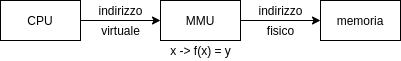
\includegraphics[width=250px]{images/9_Gestione_della_memoria/mmu.png}
\end{figure}

Supponiamo che la MMU si occupi di tradurre gli indirizzi semplicemente traslandoli di un certo offset.
Per eseguire ciò ci bastano due registri interni alla MMU:
\begin{itemize}
    \item registro base: indica di quanto si deve shiftare tutto lo spazio di memoria
    \item registro limite: indica quanto è grande lo spazio di memoria del processo corrente.
    Si usa per controllare che gli indirizzi richiesti siano effettivamente associati al processo, se così non fosse lanciamo un'eccezione da far gestire al sistema operativo.
\end{itemize}
La traduzione è effettuata con il seguente algoritmo:
\begin{itemize}
    \item se l' indirizzo virtuale è minore del contenuto del registro limite ok, altrimenti si lancia una eccezione
    \item si somma all' indirizzo virtuale il contenuto del registro base e si accede alla memoria
\end{itemize}

\subsection{Organizzazione della memoria virtuale}
\subsubsection{Memoria virtuale unica}
E' una organizzazione che prevede che tutte le diverse parti della memoria del processo siano inserite una appresso all' altra: codice, dati, stack siano tutte in un unico blob di memoria.

Questo approccio funziona ma è poco flessibile:
\begin{itemize}
    \item essendo tutte le porzioni assieme potrebbe essere difficile trovare una porzione di memoria contigua abbastanza grande che possa ospitarle per intero
    
    \item se si volessero condividere porzioni di memoria non lo si potrebbe fare in quanto bisognerebbe condividere l' intero indirizzo di base
\end{itemize}

\begin{figure}[H]
    \centering
    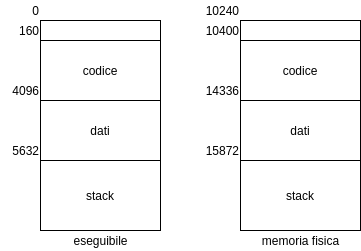
\includegraphics[width=250px]{images/9_Gestione_della_memoria/spazio_unico.png}
\end{figure}

\subsubsection{Memoria virtuale segmentata}
All' interno dello spazio virtuale del programma delimitiamo 3 segmenti diversi:
\begin{itemize}
    \item segmento codice
    \item segmento stack
    \item segmento dati
\end{itemize}
Posizioniamo ogni porzione in una zona di memoria diversa e teniamo le 3 basi.
Ogni indirizzo adesso sarà composto dal numero di segmento e dall' offset all' interno di quel segmento.
\begin{figure}[H]
    \centering
    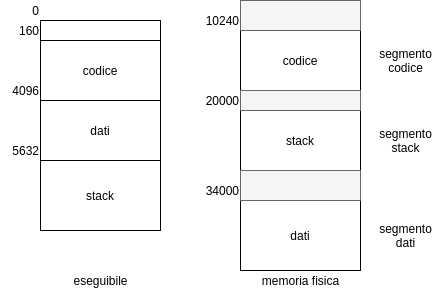
\includegraphics[width=270px]{images/9_Gestione_della_memoria/spazio_segmentato.png}
\end{figure}

Nella memoria segmentata possiamo usare un caricatore rilocante, tuttavia questa volta non deve sommare sempre la stessa base, ad esempio: se il segmento codice vuole caricare dati dovrà sommare all' indirizzo nell' istruzione la base del segmento dati.
I problemi della rilocazione statica continuano a rimanere ma almeno in questo modo abbiamo delle porzioni di memoria più piccole, è quindi più semplice trovare memoria libera.

Possiamo altresì usare la rilocazione dinamica, la MMU questa volta ha 3 coppie di registri base e limite in quanto si deve tradurre per 3 segmenti diversi da usare in casi diversi.

Si noti che se teniamo la divisione in codice, stack e dati allora non ci serve modificare il caricatore per aggiungere il numero di segmento ai vari indirizzi rilocati.
Questo perché possiamo farci furbi:
\begin{itemize}
    \item se siamo in fase di fetch, traduciamo l' indirizzo nel segmento codice
    \item se siamo in fase di esecuzione, traduciamo l' indirizzo nel segmento dati
    \item se eseguiamo istruzioni che coinvolgono la pila, traduciamo l' indirizzo nel segmento stack
\end{itemize}
possiamo continuare ad usare i programmi precedentemente compilati, non rompiamo la retro-compatibilità.
\\
\\
Abbiamo fatto un esempio su 3 segmenti, nulla ci vieta però di segmentare ancora di più, magari un segmento per la memoria condivisa, alcuni segmenti per alcune porzioni di codice condivise, tipo le librerie comuni a più processi, ecc.
Anche la protezione diventa più semplice in quanto possiamo aggiungere protezione in lettura, scrittura ed esecuzione sui singoli segmenti.

In questo scenario la MMU deve però avere un numero variabile di coppie di registri in quanto il numero di segmenti sarà diverso per ogni processo.
E' chiaro che questa cosa non si può fare in hardware quindi ci inventiamo una \emph{tabella dei segmenti} interrogata dall' hardware per rilocare le singole porzioni.

\subsection{Frammentazione della memoria}
Man mano che i processi nascono, evolvono e muoiono finiremo inesorabilmente a frammentare la memoria, otterremo quindi delle porzioni di memoria libere tra un processo e l'altro, spesso più piccole dello spazio che ci serve per allocare nuovi programmi.

Si potrebbe quindi pensare a compattare la memoria cioè spostare tutte vicine le zone utilizzate da processi ancora vivi e unire in un grande chunk le zone libere:
\begin{figure}[H]
    \centering
    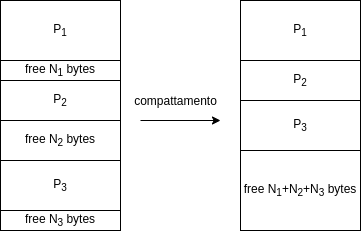
\includegraphics[width=250px]{images/9_Gestione_della_memoria/compattamento.png}
\end{figure}
questo tuttavia si può eseguire solo se la rilocazione è dinamica!

\subsection{Allocazione della memoria fisica}
Possiamo avere:
\begin{itemize}
    \item allocazione contigua: tutto il contenuto di un segmento lo inseriamo in memoria fisica in maniera contigua
    \item allocazione non contigua: il contenuto di un segmento lo inseriamo in memoria fisica a blocchi, non per forza contigui.
    Ogni blocco viene tradotto singolarmente tramite una mappa di associazione indirizzo virtuale - indirizzo fisico.
    Questi blocchi prendono il nome di pagine, hanno una dimensione fissa scelta a priori.
\end{itemize}
Tramite la allocazione non contigua risolviamo il problema della frammentazione esterna, cioè lo spazio libero tra le memorie di due processi, perché non ci serve una zona contigua, ci servono delle zone libere e basta.

Può andare di pari passo con la segmentazione, si parla di segmentazione paginata.

\subsection{Dimensioni della memoria virtuale}
\begin{itemize}
    \item caricamento unico: spazio virtuale minore o uguale a quello della memoria fisica
    
    \item caricamento a domanda: spazio virtuale superiore a quello della memoria fisica
\end{itemize}
Il caricamento unico sarebbe bello ma significa avere abbastanza memoria fisica per fare ciò che ci serve, non sempre è il caso.
Per ottenere il caricamento a domanda si implementano meccanismi di swap.

\subsection{Tecniche di gestione della memoria}
\begin{figure}[H]
    \centering
    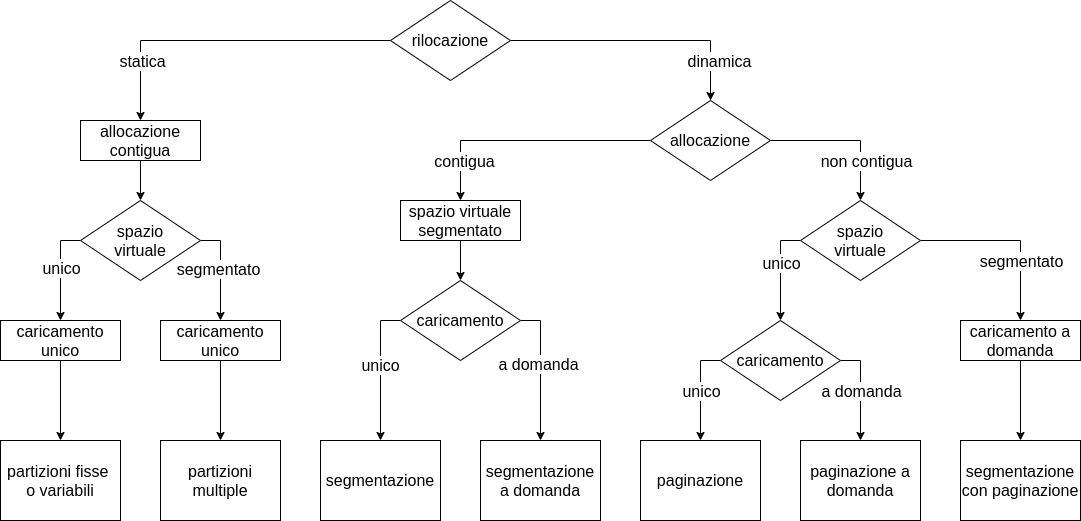
\includegraphics[width=330px]{images/9_Gestione_della_memoria/gestione_della_memoria.png}
\end{figure}

\subsubsection{Partizioni fisse}
Abbiamo rilocazione statica, allocazione contigua, spazio virtuale unico e caricamento unico.
Si suddivide lo spazio di memoria in delle partizioni di dimensioni fisse:
\begin{figure}[H]
    \centering
    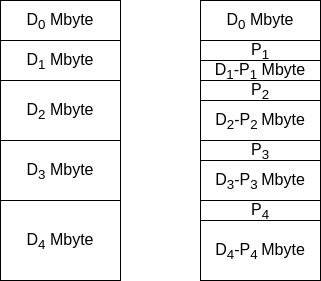
\includegraphics[width=150px]{images/9_Gestione_della_memoria/partizioni_fisse.png}
\end{figure}
Inseriamo un processo in ogni partizione e la partizione è ad uso esclusivo di quel processo.

Un problema di questo tipo di allocazione è che la frammentazione interna è molto grande in quanto i processi non occupano tutto lo spazio a loro riservato e questo spazio in più non è utilizzabile per altri scopi.

Possiamo inserire più processi su una stessa partizione se creiamo una coda per ogni partizione.
Usando il meccanismo dello swapping possiamo fare swap-out della partizione ed allocarvi sopra un nuovo processo, successivamente fare swap-in e ritornare al processo originale.

\subsubsection{Partizioni variabili}
Abbiamo rilocazione statica, allocazione contigua, spazio virtuale unico e caricamento unico.
Si suddivide lo spazio di memoria in partizioni grandi quanto servono, quindi con grandezza variabile in base alla necessità:
\begin{figure}[H]
    \centering
    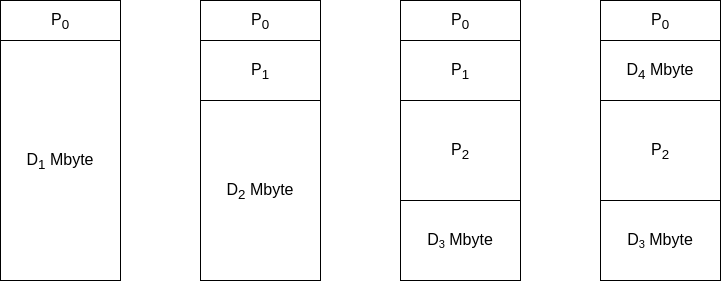
\includegraphics[width=300px]{images/9_Gestione_della_memoria/partizioni_variabili.png}
\end{figure}
Man mano che i processi nascono e si evolvono finiremo ad avere partizioni sempre più piccole, fino ad avere una frammentazione interna, cioè dei frammenti piccoli qua e la che presi singolarmente non sono utili ad allocare processi ma messi assieme sarebbero abbastanza grandi.

Un altro problema è il fatto che le partizioni libere adiacenti andrebbero detectate ed unite tra di loro per formare chunk liberi più grandi, quindi aumenta l' overhead al rilascio della memoria.

Non possiamo usare delle code per gestire l' accesso alle partizioni in quanto la dimensione è intrinsecamente legata al processo stesso, non possiamo quindi utilizzare lo swapping.

Un punto cruciale per la riduzione dell' overhead di questa gestione riguarda l' ordine che diamo alla lista delle partizioni libere:
\begin{itemize}
    \item Best-fit: fra tutte le partizioni grandi abbastanza per allocare il processo prendiamo quella più piccola.
    Ci permette di limitare la frammentazione esterna.
    Con questa tecnica la fusione delle partizioni libere adiacenti è costosa perché bisogna eseguire una ricerca esaustiva non avendo la lista ordinata per indirizzo
    
    \item First-fit: fra tutte le partizioni grandi abbastanza per allocare il processo prendiamo quella con indirizzo più basso.
    Ci permette di eseguire le fusioni al rilascio della memoria molto più velocemente.
    
    Limita anche la frammentazione esterna in quanto non cercando le partizioni più piccole non ricadiamo nella creazione di partizioni piccolissime e quindi inutili per qualsiasi scopo.
\end{itemize}

\subsubsection{Frammentazione}
In definitiva:
\begin{itemize}
    \item frammentazione interna: frazione delle partizioni non usata nella tecnica delle partizioni fisse.
    E' la differenza tra la somma delle dimensioni delle partizioni allocate e la somma delle dimensioni effettive dei processi.

    \item frammentazione esterna: frazione della memoria non utilizzata nella tecnica delle partizioni variabili.
    E' la somma delle partizioni libere che non sono grandi abbastanza da soddisfare alcuna richiesta di memoria.
\end{itemize}

\subsubsection{Partizioni multiple}
Costruiamo delle partizioni variabili in dimensione e dividiamo lo spazio di memoria del processo in segmenti in base ai diversi utilizzi della memoria.

\subsubsection{Segmentazione}
Abbiamo rilocazione dinamica, allocazione contigua, spazio virtuale segmentato e caricamento unico.

La segmentazione prevede che gli indirizzi virtuali siano composti da due coordinate: $<segmento, offset>$, ogni processo ha quindi una tabella all' interno della quale sono elencati i vari segmenti concessi al processo con l' indirizzo \emph{base} del segmento e la dimensione detta \emph{limite}.

Quando si carica un processo vanno popolati i registri che gestiscono la traduzione:
\begin{itemize}
    \item STBR - Segment Table Base Register: contiene l' indirizzo della tabella dei segmenti
    \item STLR - Segment Table Length Register: contiene le dimensioni della tabella dei segmenti
\end{itemize}
Questa tabella dei segmenti è una struttura in memoria centrale utilizzata dallo stesso hardware, fa anche parte di quelle strutture usate dal processo, va pertanto creata alla creazione del processo e distrutta alla sua uccisione.
Deve anche stare in memoria principale mentre il processo è in esecuzione.

La traduzione avviene secondo questo schema a blocchi:
\begin{figure}[H]
    \centering
    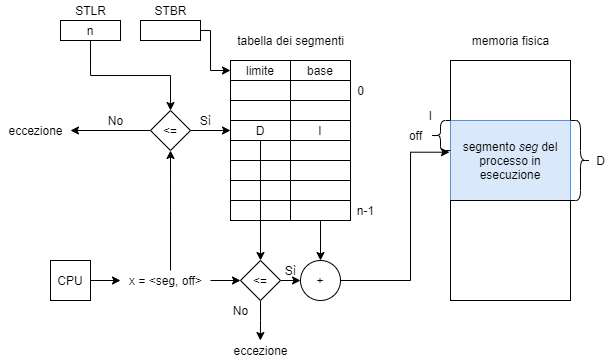
\includegraphics[width=330px]{images/9_Gestione_della_memoria/segmented_memory_mmu.png}
\end{figure}
Quando la CPU emette un indirizzo il numero di segmento viene comparato con il contenuto di STLR, se risulta maggiore allora si ha un eccezione in quanto si vuole accedere ad un segmento che non esiste nel processo.
Altrimenti si accede alla tabella dei segmenti, tramite l' indirizzo nel registro STBR, e si prelevano il limite e la base.
Il limite viene comparato con l' offset dell' indirizzo virtuale, se questo risulta maggiore allora si ha una eccezione in quanto si vuole accedere ad un offset non presente nel segmento.
Altrimenti si somma l' offset alla base e si ottiene l' indirizzo effettivo in memoria fisica.


Dato che siamo nel caso di caricamento unico la tabella viene popolata pienamente all' inizio della vita del processo, i singoli \emph{descrittori del segmento} sono così composti:
\begin{figure}[H]
    \centering
    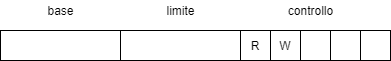
\includegraphics[width=200px]{images/9_Gestione_della_memoria/segment_record_1.png}
\end{figure}
\begin{itemize}
    \item in base si pone l' indirizzo di inizio del segmento in memoria fisica
    \item in limite si pone la dimensione in byte del segmento
    \item il campo controllo è composto da alcuni bit da vedere singolarmente:
    \begin{itemize}
        \item R: indica se quel segmento può essere letto
        \item W: indica se quel segmento può essere scritto
    \end{itemize}
\end{itemize}

Dal momento che la traduzione passa per l' accesso in memoria per ritirare le informazioni nei record si ha un notevole overhead ogni volta che la CPU emette un indirizzo.
Per limitare questo overhead possiamo ricorrere ad una cache per gli indirizzi: \emph{Translation Look-aside Buffer}, in questo modo si limita dell' 80\% l'overhead di traduzione.

\subsubsection{Segmentazione su domanda}
Se permettiamo il caricamento su domanda dobbiamo prevedere altri stati per il processo:
\begin{figure}[H]
    \centering
    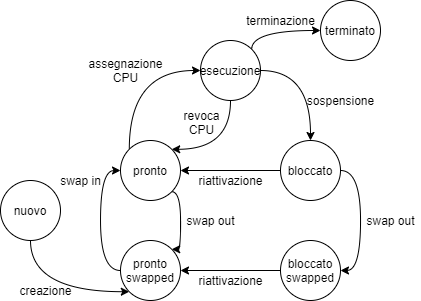
\includegraphics[width=330px]{images/9_Gestione_della_memoria/process_evolution_with_swap.png}
\end{figure}
\begin{itemize}
    \item pronto swapped: processo pronto per essere eseguito ma la cui memoria non è ancora stata caricata in memoria centrale.
    Si deve eseguire swap-in per andare in pronto
    \item bloccato swapped: processo bloccato la cui memoria è stata revocata e portata in memoria di massa
\end{itemize}
NB: si noti che se questa evoluzione del processo dovesse portare a troppo overhead si potrebbe eliminare la transizione da pronto a pronto-swapped in quanto è più conveniente fare swap-out su processi bloccati, che comunque non hanno tutte le risorse per andare avanti e dovrebbero aspettare, che eseguirlo su processi pronti che potrebbero ripartire da un momento all' altro.

Il descrittore del segmento con la segmentazione su domanda si compone di altri campi aggiuntivi usati per gestire anche il caso in cui il segmento si trovi in memoria di massa:
\begin{figure}[H]
    \centering
    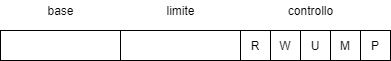
\includegraphics[width=200px]{images/9_Gestione_della_memoria/segment_record_2.png}
\end{figure}
\begin{itemize}
    \item U: bit di utilizzo, viene automaticamente settato ad 1 quando la CPU genera un indirizzo virtuale nel segmento, quindi al primo accesso.
    E' usato per statistiche in alcuni algoritmi di swapping

    \item M: bit di modifica, viene automaticamente settato ad 1 quando si accede al segmento in scrittura.
    E' usato per decidere se allo swap-out bisogna ricopiare il segmento e sostituire la copia già presente in memoria di massa. Se non è stato modificato è inutile sovrascrivere la copia che già si ha.

    \item P: bit di presenza in memoria, se è ad 1 il segmento è presente in memoria centrale, altrimenti si trova su disco.
    Se P=0 il contenuto del campo base indica l' indirizzo su disco al quale trovare la copia del segmento swappato.
\end{itemize}

NB: il diagramma della traduzione visto precedentemente deve essere modificato: si deve aggiungere il controllo sul bit P in quanto se P=0 allora si ha un segfault, nella gestione di questa eccezione si deve ricaricare il segmento mancante e poi far ripartire il processo dall' istruzione che ha causato l' eccezione.

NB: il caricamento su domanda se non eseguito correttamente può portare a problemi: supponiamo di avere due segmenti che si puntano a vicenda e di poter caricare solo uno dei due segmenti per volta, quando eseguiamo codice dal primo abbiamo un segfault perché non riesce ad accedere al secondo segmento, allora lo allochiamo al posto del primo, torniamo a rieseguire il codice, ma ora non è più presente il segmento codice, quindi lo ricarichiamo sopra quello dati e così via.
Alla fine non riusciamo ad andare avanti perché ci servono i due segmenti contemporaneamente presenti in memoria centrale.

\subsubsection{Paginazione}
Abbiamo rilocazione dinamica, allocazione non contigua, spazio virtuale unico, caricamento unico.

Suddividiamo lo spazio di indirizzamento virtuale in blocchi di indirizzi di dimensioni fisse, chiamiamo questi blocchi \emph{pagine}.
Suddividiamo lo spazio fisico in blocchi di indirizzi delle stesse dimensioni delle pagine, chiamiamo questi blocchi \emph{frame}.

Ogni pagina viene allocata in un diverso frame, finché ci sono frame liberi.
Con questo mapping 1 ad 1 possiamo avere pagine consecutive che all' atto pratico sono tradotte su frame non necessariamente consecutivi.
Per fare questo ci serve tuttavia una tabella di traduzione detta \emph{tabella delle pagine}.
\begin{figure}[H]
    \centering
    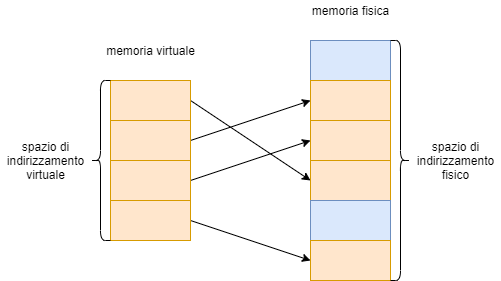
\includegraphics[width=280px]{images/9_Gestione_della_memoria/pagination_example.png}
\end{figure}
Di fatto gli indirizzi nella stessa pagina sono contigui, i blocchi non è detto.

Per attuare questa traduzione ci servono gli indirizzi a due dimensioni, composti dal numero di pagina e dall' offset all' interno della pagina.
Supponiamo che una pagina abbia 1Kb di dimensione, allora i 10 bit più bassi sono usati come offset nella pagina mentre la restante parte vanno ad indicare il numero di pagina.
Di fatto ci bastano i normali indirizzi, l' hardware poi può suddividere l' indirizzo nelle due porzioni in autonomia.
\begin{figure}[H]
    \centering
    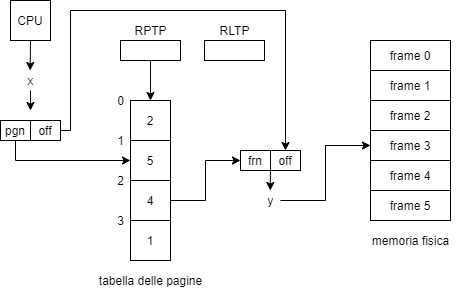
\includegraphics[width=330px]{images/9_Gestione_della_memoria/pagination_mmu.png}
\end{figure}
Quando la CPU emette un indirizzo esso viene suddiviso in indirizzo di pagina ed offset nella pagina.
Tramite il registro della CPU RPTP si può accedere alla tabella delle pagine del processo corrente, quindi ritirare il numero di frame associato alla pagina ricercata.
Una volta preso il numero del frame concateniamo lo stesso offset dell' indirizzo richiesto ed otteniamo l' indirizzo in memoria fisica.

Ovviamente se il numero di pagina è più grande del contenuto di RLTP si ha una eccezione perché si sta chiedendo di accedere ad una pagina non associata al processo.

Anche qui per abbattere il numero di accessi in memoria per tradurre gli indirizzi si usa una cache interna alla MMU, parliamo anche qui di TLB - translation lookaside buffer.

Ci serve anche una struttura che ci elenchi tutti i frame liberi, la chiamiamo \emph{frame table} e la costruiamo come una coda circolare.

\subsubsection{Paginazione a domanda}
Abbiamo rilocazione dinamica, allocazione non contigua, spazio virtuale unico, caricamento a domanda.

Non allochiamo tutto lo spazio del processo all' avvio, lo allochiamo eventualmente su alcuni page fault.
Il record della tabella delle pagine è così composto:
\begin{figure}[H]
    \centering
    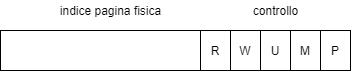
\includegraphics[width=200px]{images/9_Gestione_della_memoria/page_record.png}
\end{figure}
\begin{itemize}
    \item nell' indice della pagina inseriamo l' indice del frame mappato su quella pagina se P=1, altrimenti inseriamo l' indirizzo su disco di dove abbiamo salvato la pagina per fare swap-out
    \item R, W: sono i permessi di lettura e scrittura sulla pagina
    \item M: bit di modifica settato ad 1 la prima volta che si fa una scrittura su quella pagina
    \item U: bit di uso settato ad 1 al primo accesso alla pagina
    \item P: bit di presenza, indica se la pagina si trova nella memoria centrale
\end{itemize}
Se si prova ad accedere ad un indirizzo in una pagina con P=0 si ha un page-fault, in genere l' handler di questa eccezione si occupa di fare swap-in della pagina mancante.

Si noti che l' utilizzo della paginazione porta ad una frammentazione interna in quanto all' interno della pagina potrei avere degli sprechi, cioè memoria in una pagina associata ad un processo ma inutilizzata.
Per limitare questo spreco posso creare pagine piccole, ma finirei ad avere una tabella delle pagine più grande della memoria stessa, quindi si convive con un po' di spreco.

\subsubsection{Segmentazione paginata}
Abbiamo rilocazione dinamica, allocazione non contigua, spazio virtuale segmentato e caricamento a domanda.
Costruiamo la struttura della segmentazione su pagine, quindi il codice emette indirizzi virtuali nello spazio dei segmenti che poi vengono tradotti nelle singole pagine nella memoria fisica.

\begin{figure}[H]
    \centering
    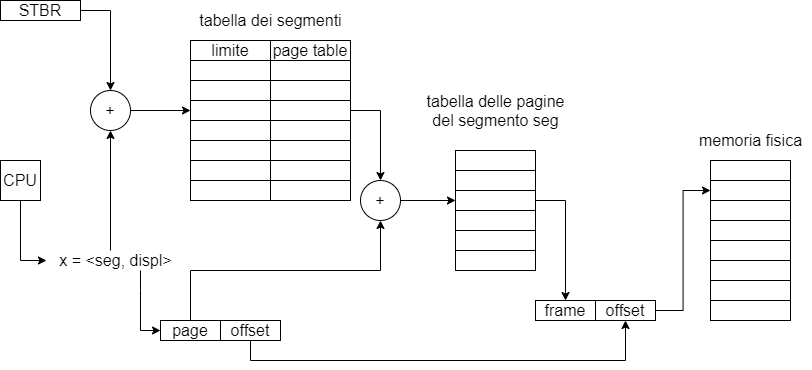
\includegraphics[width=330px]{images/9_Gestione_della_memoria/segmentazione_paginata.png}
\end{figure}
Per implementare questa politica ci servono i bit di presenza sia sulla pagina che sul segmento in quanto potremmo avere segmenti caricati solo per alcune pagine così come potremmo avere interi segmenti non caricati, se il bit di presenza del segmento è 0 la tabella delle pagine non è in memoria, va quindi creata se è la prima volta oppure ricaricata dalla swap.

Nella tabella dei segmenti ogni descrittore di segmento contiene il limite e l' indirizzo di una tabella delle pagine.

In questa configurazione dobbiamo fare ben due accessi in memoria per avere il contenuto della memoria fisica, anche in questo caso per ottimizzare si usa una TLB che mette in cache le traduzioni degli indirizzi.

\subsubsection{Paginazione a due livelli}
La tabella delle pagine potrebbe essere troppo grande da allocare in memoria per tradurre tutte le pagine.
Ci inventiamo quindi una tabella divisa in 2 livelli:
la CPU genera un indirizzo virtuale costituito da due numeri di pagina virtuale ed un offset, usiamo il primo numero di pagina per accedere alla prima tabella, qui troviamo l' indirizzo della tabella di secondo livello.
In questa seconda tabella accediamo al secondo numero di pagina virtuale dell' indirizzo e qui vi troviamo il numero di frame.
Al numero di frame concateniamo l'offset dell' indirizzo virtuale ed abbiamo l' indirizzo fisico completo.

\begin{figure}[H]
    \centering
    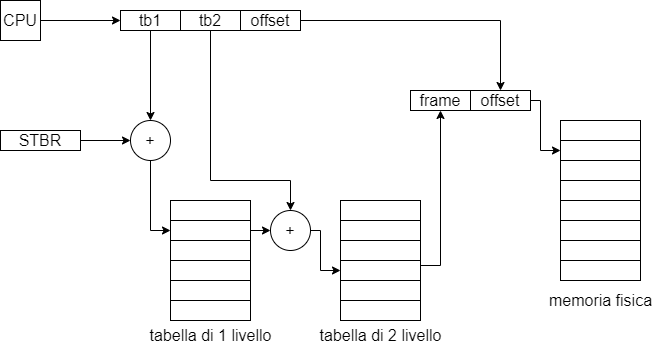
\includegraphics[width=300px]{images/9_Gestione_della_memoria/paginazione_due_livelli.png}
\end{figure}

Con questa logica speziamo una tabella grande in tante più piccole che possiamo allocare o non allocare all' occorrenza.


\subsubsection{Spazio del sistema operativo}
Per far si che il sistema operativo possa accedere al suo codice è necessario mappare lo spazio di memoria in tutti i processi, quindi nella tabella dei segmenti di ogni processo ci sarà sempre il segmento relativo al sistema operativo.
Per gestire la protezione possiamo pensare di inserire i privilegi all' interno dei bit di flag del descrittore di segmento.


\subsection{Gestione di un page-fault}
Il processo emette un indirizzo, si accede alla tabella delle pagine del processo in esecuzione, il record della pagina cercata ha P=0, si ha un page-fault.
Si cerca nella tabella delle pagine fisiche un frame libero quindi si prende l' indirizzo della pagina cercata nella swap area e si ricopia il contenuto dalla swap verso il frame libero.
Una volta finita la copia si inserisce nel record della tabella delle pagine l' indirizzo fisico del frame che si sta occupando, facendolo diventare di fatto parte della memoria del processo.
In fine si rimette in esecuzione il processo dalla stessa istruzione che ha causato il fault.

Si noti che la copia da disco a memoria può essere fatta con DMA quindi in maniera asincrona rispetto alla CPU, il momento perfetto per mandare il processo faulted in pausa è proprio dopo aver avviato il trasferimento.

NB: si noti che da quando il processo viene stoppato a quando il processo viene rimesso in esecuzione ci saranno altri processi a prendere controllo della CPU.
Questi processi possono fare di tutto, quindi ad esempio avere altri page-fault e portare a rimpiazzare la pagina appena caricata con altre.
Succede se ho un brutto algoritmo di rimpiazzamento ma non c'è la certezza che una volta messo in esecuzione il processo potrà effettivamente andare avanti senza problemi.

\subsection{Rimpiazzamento delle pagine}
Se al page-fault non trovo un frame libero devo cercare un frame da liberare per fare spazio ad un frame del processo corrente.

Per fare ciò devo innanzitutto cercare uno slot libero nella swap, una volta trovato vi copio sopra il frame del processo target da liberare, aggiorno dunque la sua tabella delle pagine ponendo P a 0 e sostituendo l' indirizzo della pagina con l' indirizzo del frame nella swap.
In fine aggiorno la tabella delle pagine del processo corrente e lo faccio ripartire.
In tutto questo devo anche aggiornare la tabella delle pagine fisiche in quanto un frame ha cambiato processo che lo possiede.

Ci serve un criterio, un algoritmo, per scegliere quale pagina di quale processo revocare e sostituire.
Inoltre sarebbe bello scegliere queste pagine in modo che non mi impediscano di far andare avanti altri processi.
Definiamo quindi il concetto di \emph{Working-Set} cioè l' insieme delle pagine correntemente utilizzate da un processo.
Inizialmente tende a crescere con l' evoluzione del programma, ma poi tende a stabilizzarsi in quanto le sezioni di codice si stabilizzano ed anche le strutture dati utilizzate.
Il working set non è quindi l' insieme delle pagine con il bit di utilizzo ad 1 ma lo useremo come approssimazione.

Posso usare due strategie di rimpiazzamento:
\begin{itemize}
    \item rimpiazzamento \emph{locale}: per allocare una pagina ne rimuovo un' altra dallo stesso processo
    \item rimpiazzamento \emph{globale}: per allocare una pagina ne rimuovo un' altra da un processo qualsiasi
\end{itemize}

\subsubsection{Trashing}
Un sistema finisce in \emph{trashing} quando passa la stragrande maggioranza del tempo a gestire i page-fault.
Questo succede quando si opta per un cattivo algoritmo di rimpiazzamento e si rimpiazzano pagine in realtà molto utilizzate.

\subsubsection{Algoritmo ottimo}
Sarebbe bello rimpiazzare le pagine che di sicuro non saranno più accedute in futuro.
Questo algoritmo tuttavia è impossibile perché non possiamo conoscere il futuro e quindi gli accessi in memoria del processo.

\subsubsection{Algoritmo FIFO}
Dato che abbiamo deciso di implementare la tabella delle pagine fisiche come una coda circolare possiamo scorrerla in avanti all' infinito.
Quando c'è un page-fault proviamo a prendere il prossimo frame libero, se non ce ne sono vuol dire che abbiamo scorso tutta la coda circolare e siamo tornati all' inizio.
Decidiamo quindi di rimpiazzare proprio la pagina puntata in questo momento dall' indice di questa coda circolare.
All' atto pratico andiamo a rimpiazzare le pagine che sono da più tempo in memoria.

Non è ovviamente un algoritmo ottimale in quanto potrei rimuovere pagine che sono spesso riferite da un processo, però ci guadagno in semplicità e quindi in overhead.

Si noti che usare disciplina FIFO in aggiunta al rimpiazzamento locale le probabilità di fare una pessima scelta sono più alte.

\subsubsection{Algoritmo Least Recently Used}
Rimpiazziamo la pagina meno recentemente utilizzata.
Per fare ciò ci serve un modo per loggare gli accessi, supponiamo di aggiungere un campo \emph{timestamp} in ogni record della pagina, ci servono almeno 32 bit di timestamp in modo da avere granularità dei microsecondi.
Stiamo quindi raddoppiando la dimensione di ogni record, inoltre aggiungiamo un grande overhead in quanto ogni volta che si esegue un accesso in una pagina bisogna generare il timestamp dell' accesso ed aggiornare quello già presente.

\subsubsection{Algoritmo second-chance}
E' un algoritmo a rimpiazzamento locale.
Supponiamo di avere le pagine allocate per un processo, ognuna con il suo bit di uso.
Organiziamo queste pagine in una coda circolare e manteniamo un puntatore detto \emph{vittima} che all' inizio punti alla pagina 1.

Al momento del page-fault controlliamo la coda partendo dalla pagina puntata da vittima, confermiamo la vittima se il suo bit di utilizzo è a 0.
Se invece la pagina puntata da vittima ha il bit ad 1 lo setto a 0 e scorro al prossimo record nella coda.

Si noti che se tutte le pagine hanno il bit di uso a 1 dopo un primo giro completo della coda circolare tutti saranno settati a 0, quindi la vittima confermata non è altro che la prima della lista, esattamente come FIFO.

E' un approccio ibrido rispetto a FIFO ed LRU che aggiunge poco overhead.

Una ottimizzazione che potrei fare all' algoritmo è controllare anche il bit di modifica, se scelgo una vittima con modifica a 0 mi risparmio l' overhead di salvare la pagina in swap potendomi rifare alla copia che già ho.

\begin{figure}[H]
    \centering
    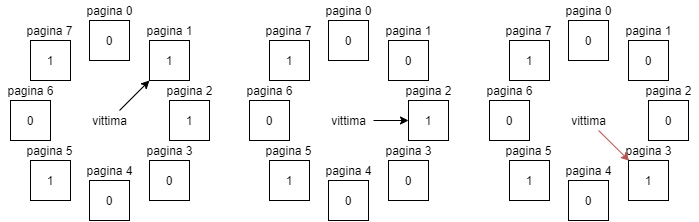
\includegraphics[width=330px]{images/9_Gestione_della_memoria/second_chance.png}
\end{figure}

